\documentclass[11pt]{article}

\usepackage{graphicx} %so this is for the pictures
\usepackage{amsmath} %this is for the equations
\usepackage{xr} %and this is for refer the labels inside the SI file

% load the numbers from py code
\newcommand{\testaccuracy}{92.3}
\newcommand{\npatients}{520}
\newcommand{\percentpositive}{61.5}


% to refer the labels from SI.tex
\externaldocument{si}

\title{Predicting Early-Stage Diabetes from Symptoms: A Toy Workflow Example}
\author{Nur Ceren Kabakci}
\date{\today}

\begin{document}
\maketitle

\begin{abstract}
    This paper shows a reproducible workflow. A logistic regression model predicts diabetes from symptoms with \testaccuracy\% accuracy on unseen patients.

\end{abstract}

\section{Introduction}
\label{sec:intro}
Early detection od diabetes can improve patient outcomes. We use the symptom survey dataset of \cite{islam2020}, which has
\npatients{} patients, of whom \percentpositive\% have diabetes.

\section{Methods}
\label{sec:methods}

\subsection{Data}
Each patient has an age, a gender and 14 yes/no symptoms. Details of the data are given in Section~\ref{sec:si-data} of the SI.

\subsection{Model}
I fit a logistic regression model, implemented in scikit-learn \cite{pedregosa2011}. It is described by
\begin{equation}
    P(\text{diabetes}=1 \mid x) = \frac{1}{1 e^{-(+ b_0 + b_1 x_1 + \dots b_p x_p)}},
    \label{eq:logistic}
\end{equation}
where $x_1,\dots,x_p$ are the predictors and $b_0,\dots,b_p$ are coefficients
learned from the data. Equation~\ref{eq:logistic} is the model used in
Section~\ref{sec:results}.

\section{Results}
\label{sec:results}
I trained on 80\% of patients and tested on the remaining 20\%. The test accuracy was \testaccuracy\%.
Figure~\ref{fig:coef} shows the fitted coefficients; larger positive values mean that symptom raises the predicted chance of diabetes.

\begin{figure}[ht]
    \centering
    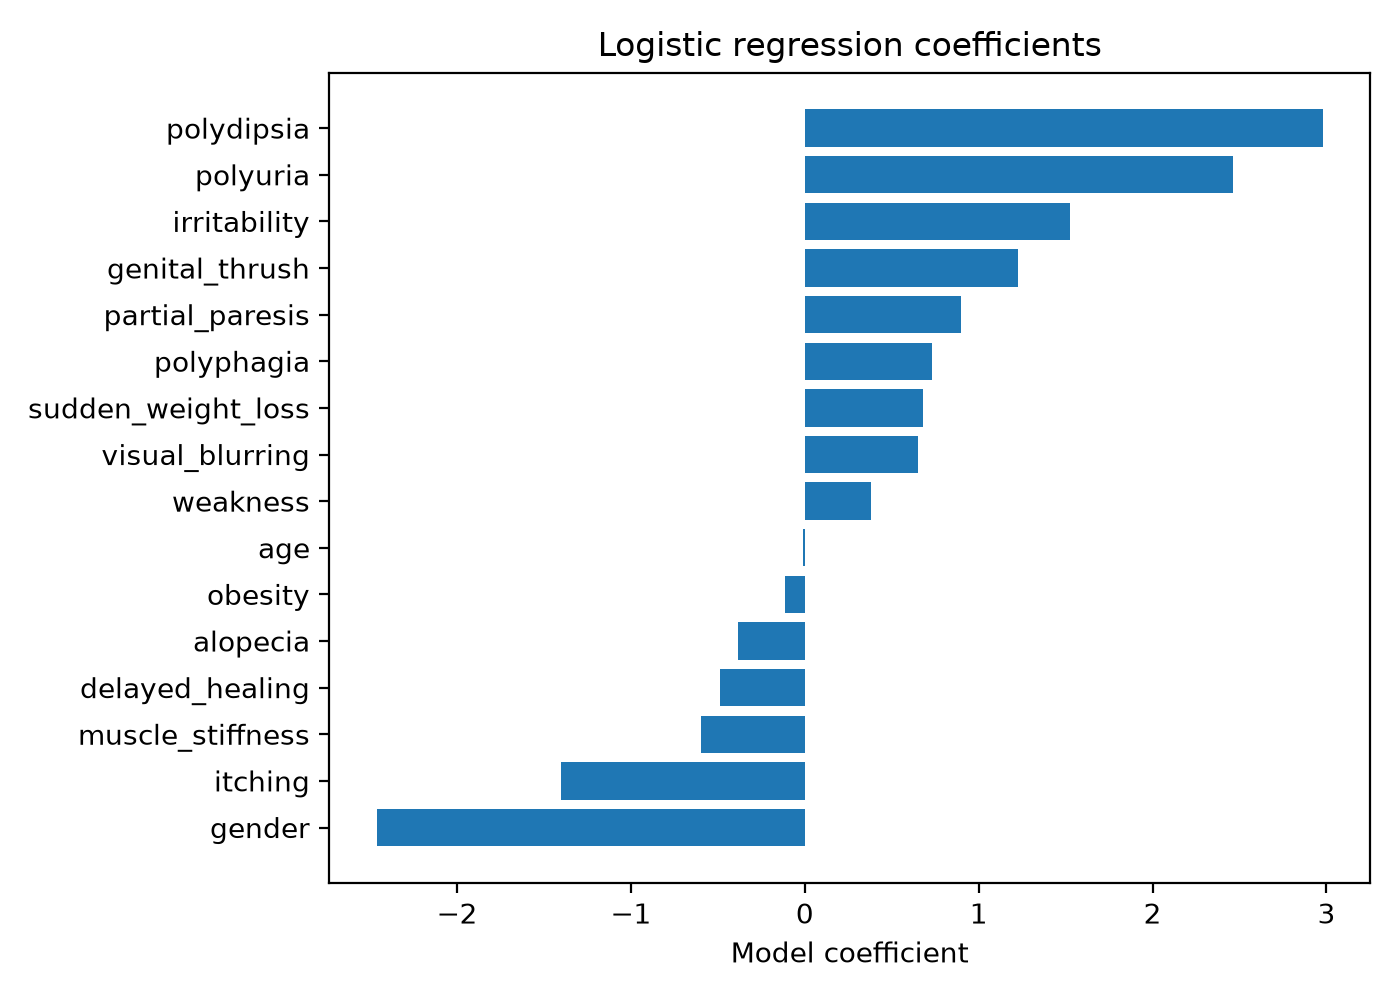
\includegraphics[width=0.8\textwidth]{../results/coefficients.png}
    \caption{Coefficients of the logistic regression model. Positive bars
  increase the predicted probability of diabetes.}
  \label{fig:coef}
\end{figure}

\section{Discusion}
This was a simple analysis and results may change with other models. More detail on the data is in Section~\ref{sec:si-data} of SI.

\bibliographystyle{plain}
\bibliography{refs}

\end{document}